\documentclass{beamer}

%% Juego de caracteres usado en el archivo fuente: UTF-8
\usepackage{ucs}
\usepackage[utf8x]{inputenc}
\uselanguage{spanish}
%Para la identación del español
\usepackage[spanish]{babel}
\usepackage{animate}

% There are many different themes available for Beamer. A comprehensive
% list with examples is given here:
% http://deic.uab.es/~iblanes/beamer_gallery/index_by_theme.html
% You can uncomment the themes below if you would like to use a different
% one:
%\usetheme{AnnArbor}
%\usetheme{Antibes}
%\usetheme{Bergen}
%\usetheme{Berkeley}
%\usetheme{Berlin}
%\usetheme{Boadilla}
%\usetheme{boxes}
%\usetheme{CambridgeUS}
%\usetheme{Copenhagen}
%\usetheme{Darmstadt}
%\usetheme{default}
%\usetheme{Frankfurt}
%\usetheme{Goettingen}
%\usetheme{Hannover}
%\usetheme{Ilmenau}
%\usetheme{JuanLesPins}
%\usetheme{Luebeck}
\usetheme{Madrid}
%\usetheme{Malmoe}
%\usetheme{Marburg}
%\usetheme{Montpellier}
%\usetheme{PaloAlto}
%\usetheme{Pittsburgh}
%\usetheme{Rochester}
%\usetheme{Singapore}
%\usetheme{Szeged}
%\usetheme{Warsaw}

%Para la identación del español
\usepackage[spanish]{babel}

\title{Fantasy}

% A subtitle is optional and this may be deleted
%\subtitle{Optional Subtitle}

\author{\textcolor{white}{Stimey}}
% - Give the names in the same order as the appear in the paper.
% - Use the \inst{?} command only if the authors have different
%   affiliation.

%\institute[Escuela Superior de Ingeniería] % (optional, but mostly needed)
%{
%  \inst{1}%
%  Department of Computer Science\\
%  University of Somewhere
%  \and
%  \inst{2}%
%  Department of Theoretical Philosophy\\
%  University of Elsewhere}
% - Use the \inst command only if there are several affiliations.
% - Keep it simple, no one is interested in your street address.

\date{26 de febrero de 2019}
% - Either use conference name or its abbreviation.
% - Not really informative to the audience, more for people (including
%   yourself) who are reading the slides online

%\subject{Theoretical Computer Science}
% This is only inserted into the PDF information catalog. Can be left
% out. 

% If you have a file called "university-logo-filename.xxx", where xxx
% is a graphic format that can be processed by latex or pdflatex,
% resp., then you can add a logo as follows:

% pgfdeclareimage[height=0.5cm]{university-logo}{university-logo-filename}
% \logo{\pgfuseimage{university-logo}}

% Delete this, if you do not want the table of contents to pop up at
% the beginning of each subsection:
%\AtBeginSubsection[]
%{
%  \begin{frame}<beamer>{Índice}
%    \tableofcontents[currentsection,currentsubsection]
%  \end{frame}
%}

% Let's get started
\begin{document}

\begin{frame}
  \titlepage
  \begin{center}
  Luis Gutiérrez Flores\\
Nicolás Ruiz Requejo\\
Jesús Rodríguez Heras\\
Arantzazu Otal Alberro\\
Alejandro Segovia Gallardo\\
Alejandro José Caraballo García\\
Gabriel Fernando Sánchez Reina	
  \end{center}
  
\end{frame}

%\begin{frame}{Índice}
%  \tableofcontents
%  % You might wish to add the option [pausesections]
%\end{frame}

\section{Fantasy}
\begin{frame}{Fantasy}
\begin{block}{¿Qué es?}
	Aplicación web con la finalidad de que el profesorado pueda redactar una serie de tareas (fantasías) para sus alumnos de entre 10 y 13 años para que puedan aprender de forma creativa.
	
	Los alumnos también podrán crear dichas fantasías con la finalidad de estudiar o, como tareas establecidas por el profesorado.
\end{block}
\end{frame}

\section{Workspace}
\begin{frame}{Workspace}
\begin{block}{Background}
	Ventana donde se podrá seleccionar una imagen y establecerla como fondo del workspace. También será posible añadir texto para ayudar en el aprendizaje del alumnado.
\end{block}
\begin{block}{Punto activo}
	Establece puntos activos en el workspace que podrán ser modificados al gusto del profesorado.
\end{block}
\end{frame}

\begin{frame}{Boceto}
	\begin{figure}
		\centering
		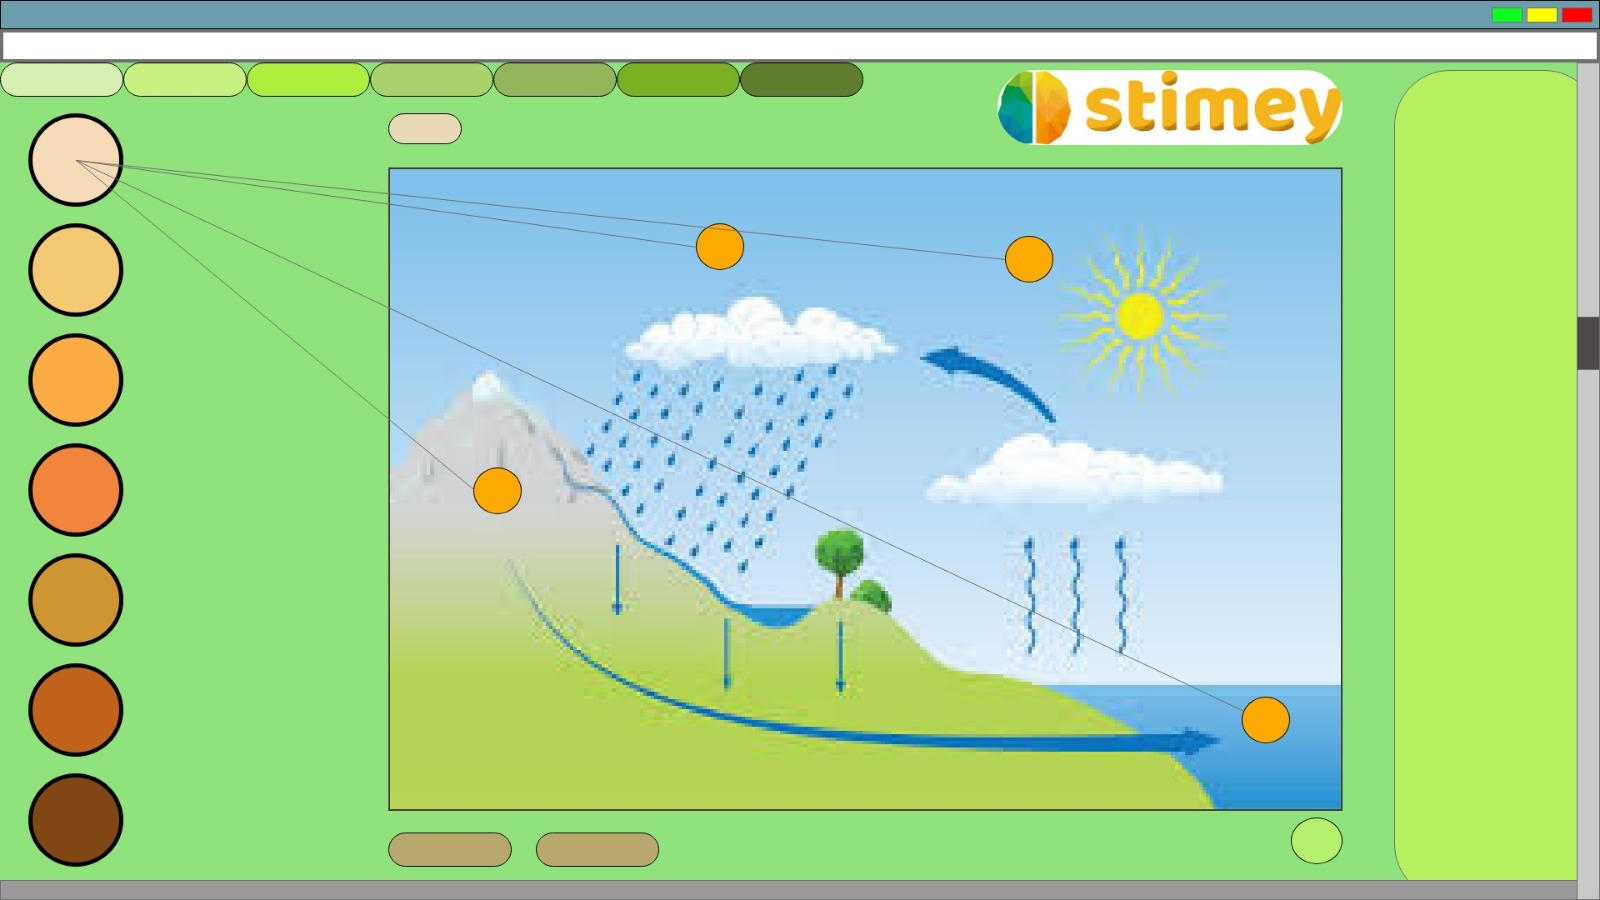
\includegraphics[scale=0.21]{Boceto.jpeg}
	\end{figure}
\end{frame}

\section{Características}
\begin{frame}{Características}
\begin{itemize}
	\item Cada punto activo finalizará con un quiz.
	\item No se podrá acceder al siguiente punto activo hasta completar el quiz del actual.
	\item Código único por fantasía.
	\item Notificación al profesorado cuando el alumnado finalice una fantasía.
	\item Públicas (por efecto) o privadas.
	\item Posibilidad de clonar fantasías.
\end{itemize}
\end{frame}
\end{document}


